\begin{problema}{Internet Bandwidth}{Standard}{Standard}{UVa} 


On the Internet, machines (nodes) are richly interconnected, and many paths may exist between a given pair of nodes. The total message-carrying capacity (bandwidth) between two given nodes is the maximal amount of data per unit time that can be transmitted from one node to the other. Using a technique called packet switching, this data can be transmitted along several paths at the same time. \\

For example, the following figure shows a network with four nodes (shown as circles), with a total of five connections among them. Every connection is labeled with a bandwidth that represents its data-carrying capacity per unit time.  \\

In our example, the bandwidth between node 1 and node 4 is 25, which might be thought of as the sum of the bandwidths 10 along the path 1-2-4, 10 along the path 1-3-4, and 5 along the path 1-2-3-4. No other combination of paths between nodes 1 and 4 provides a larger bandwidth. \\

You must write a program that computes the bandwidth between two given nodes in a network, given the individual bandwidths of all the connections in the network. In this problem, assume that the bandwidth of a connection is always the same in both directions (which is not necessarily true in the real world). \\ 


\begin{center}
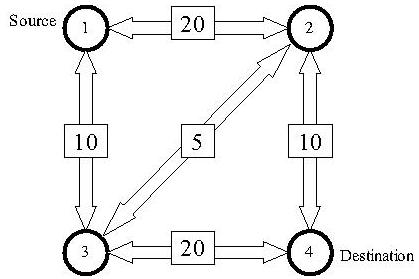
\includegraphics[height=5cm]{graficos/bandwidth}
\end{center}



\InputFile

The input file contains descriptions of several networks. Every description starts with a line containing a single integer $n$ ($2 \leq n \leq 100$), which is the number of nodes in the network. The nodes are numbered from $1$ to $n$. The next line contains three numbers $s$, $t$, and $c$. The numbers $s$ and $t$ are the source and destination nodes, and the number $c$ is the total number of connections in the network. Following this are $c$ lines describing the connections. Each of these lines contains three integers: the first two are the numbers of the connected nodes, and the third number is the bandwidth of the connection. The bandwidth is a non-negative number not greater than 1000. 

There might be more than one connection between a pair of nodes, but a node cannot be connected to itself. All connections are bi-directional, i.e. data can be transmitted in both directions along a connection, but the sum of the amount of data transmitted in both directions must be less than the bandwidth. 

A line containing the number $0$ follows the last network description, and terminates the input. 
 \\


\OutputFile

For each network description, first print the number of the network. Then print the total bandwidth between the source node $s$ and the destination node $t$, following the format of the sample output. Print a blank line after each test case.  \\


\Example

\input ejemplos/bandwidth.txt


URL: \\
http://uva.onlinejudge.org/index.php?
\\option=com\_onlinejudge\&Itemid=8\&page=show\_problem\&problem=761

\end{problema}
